%edited Sandra 270910
%tone for all words in
%tone for all this \S

\chapter{Historical and Sociolinguistic Background}
\label{sec:SOC-lingvit}


\begin{flushright}

{\C daakputii kaa dʊɔ nɪɪ nɪ,\\ ʊ wa kɪŋ bɛrɛgɪ  ɲʊg}\\[1ex]
{\it ``Even if a log lies in the water,\\ it can never change into a
crocodile''}\\[2ex]
\Source{{\it - Chakali proverb}}

\end{flushright}


\section{Introduction}
\label{sec:SOC-Intro}


This chapter introduces the Chakali among whom I stayed and provides an
overview of the current sociolinguistic situation. Since the
speakers recognize that their language is slowly disappearing, I  report on
the vitality and endangerment of the language based on the 
guidelines given in \cite{UNES03, Reco03}.   Some factors
which are causing the language to vanish, and  other factors which are
responsible
for the language to still be spoken today are assessed. The chapter starts
by introducing the
ethnographic context  to locate the speakers and their environment. Sources
vary from published materials, interviews, rumors and observations. 

% Attention is focused on aspects
% which may contribute to the understanding of the present sociolinguistic
% situation. Then, topics such as areal sociolinguistics, contact languages,
% diglossia vs.bilingualism, convergence,  linguistic vitality and endangerment
% are examined.

%The motivation behind this chapter is that on the one hand sociolinguistic
%information are always reduced to a short paragraph in descriptive
%linguistics. More is needed if one wishes to understand the 
%endangerment of a language. Language description spare the reader from useful
%information,.


\section{Ethnographic context}
\label{sec:SOC-ethno}

With `Chakali',    three concepts are identified. The term may be used  to name
a
land,  an ethnic group or a language.  However it would be wrong to think that a
member of the Chakali ethnic group  or  
someone living on Chakali land necessarily speaks the language.  Chakali may refer to the
area known as {\S tʃàkálɪ́ hàɣlɪ́ɪ̀} `Chakali soil/sand/land', or simply  {\S
tʃàkálɛ́}. The Chakali land is
defined in \cite{Daan94} on the basis of geographical boundaries: Bulenga,
Tiisa, Sogla, Tuosa, Chagu, Motigu, Ducie, Katua, Bisikan, Kandia, Dupari,
Gilan and Gurumbele (and their surrounding land) are the  thirteen communities
forming the Chakali land. The term {\S tʃàkálɪ́ɛ́} refers to the people, or the
ethnic group, in both Waali and Chakali. The singular term {\S tʃàkálóó} `a
Chakali person'  has the same signification in Waali and all Chakali villages
except for the communities  Motigu, Gurumbele, Katua and Ducie, where a
Chakali
person is referred to as {\S tʃàkálɪ́}.  Individualizing is achieved through
compounding; {\S tʃàkálbáàl}  `a Chakali man', {\S tʃàkálhã́ã̀ŋ} `a
Chakali woman'
and {\S tʃàkálbìé} `a Chakali child'. The language they speak is known as {\S
tʃàkálɪ́}. Since this work is mainly concerned with the language,  all these
concepts are captured under  \textit{Chakali},
 the term being accompanied with specification when necessary (e.g. Chakali
speaker,
Chakali land, etc.). However it is crucial to keep in mind that 
these three  concepts (i.e. land, ethnicity and language) are 
interwoven.  This is exactly
what \citeauthor{Good54} describes: 

\begin{Lquote} [t]he use of one self-applied name may cut across the linguistic
frontiers which have already been defined. The Chakalle who inhabit the eastern
part of the Wa district are split into those speaking a language of the Mossi
group and those speaking a Grusi language. ``Speaking a language" refers to the
tongue which dominates in the child's play group; the eastern Chakalle who use a
Grusi language in this context are in fact mostly bilingual. The common name for
the group derives from a recognition of uniformity in other social activities.
\end{Lquote} \Source{ \citet[2]{Good54}}


\subsection{Historical sketch}
\label{sec:SOC-hist-bk}


The history of the Grusi people, especially of the groups found today in Ghana
and
Burkina Faso before the middle of the nineteenth century, is for the most part
unknown.  \citet[13]{Mano51}  claims that ``what are now the
Northern Territories was peopled some 500 years ago by ancestors of the
present-day Tampolense, Vagala and certain Isala groups, and by some Konkomba
groups to the east''.\footnote{See also \citet[516-7]{Ratt32b}.} Based on the
maps of the divisions of the nineteenth century Gonja state
\citep{Good67, Wilk86},  Chakali villages were apparently within Katua, Daboya
or Wasipe districts. No
mention of Chakali (or Chakalle) is found in \cite{Good67, Wilk86}, nor in
\cite{Dupe84}.  

Although the oral records from different villages claim their ancestors from
different locations, what is known today as the Wa East district is the area
where Chakali is
known to have emerged. The root {\S tʃakal} and the origin of this
appellation are unknown.  The only
indication I have appears in \citet[479]{Ratt32b}, where {\S Chakal-boi} in
Sisaala refers to a place name, a hill situated  50 km north of Daboya and
close to the Tampulma village called Yabum. The elders I  met were unable
to provide an etymology, nor a story of how this group came to be named as  
they are. Looking upon the situation and considering the historical information
presented in \cite{Ratt32a, Ratt32b, Good54, Wilk89, Daan92b, Daan94, Sali08}, 
a
possible origin of the  appellation is a metonymic transfer.   The
inhabitants  became so  intimately associated with that area,  that
they become
known as one `ethnic' group. The appellation was probably subsequently
reinforced by the nineteenth century alliance with the Waala (see ChakaliWalea
({\S tʃakalwɔlɛɛ}) in \citet[63]{Daan94}).


According to \citet[77]{Daan92}, pre-colonial Chakali was a segmentary
society of independent  villages.  Each village  ({\S tɔ́ʊ̀}) constituted
a
small political
unit with its own indigenous leadership. This type of society is often called
acephalous or stateless and is characterized by its lack of centralized
authority \citep[see Group B in][5]{Fort40}. Preceding the introduction
of chieftaincy and still very much in control of local affairs today,  the
institutions of  landlordships ({\S tɔ́ɔ̀tɪ̀ɪ̀ná}), the administrative body of
elders representing the clans  ({\S nɪhɪɛ̃sa}), the soothsayers ({\S
vʊ̀vʊ̀tá}) and the
shrine 
representatives  ({\S vʊ̀gtɪ̀ɪ̀ná}) collaborate in the administration of a
community.

Inter-village network was and still is 
sustained by the co-operation of (patrilineal and matrilineal) kinship  and
common shrines.  Through this
co-operation they were able to maintain equality and peace in the communities
and  protect themselves from being brought under
centralized authority. 


As for other groups in northern Ghana, the institution of
chieftaincy was certainly known by the acephalous Chakali, but  it was imposed
on them only recently.   \cite{Wilk89, Daan94, Sali08} all seem to agree that war-chiefs  ({\S
boŋ naa})  in Chakali,  a role similar to the leader of the soldiers ({\S
mboŋwura}) in Gonja organization,  date back to the time of, and likely due to,
Samori and the
 Zabarima
slave raids.\footnote{``Zabarima occupation of Ducie occurred
probably early in May 1897.'' \cite[133]{Wilk89}} At that time the Chakali and
Waala contracted defense cooperation,
what is known as the {\S koŋboŋi} alliance \citep[63]{Daan94}. 
%b or gb ?

At the beginning of the colonial era, the British favored a  centralized
administration over the
acephalous mode of administration found in Chakali. These independent
micro-states and their distance from Wa were unmanageable unless consolidated
under  trusted men selected by the  district commissioner. The British colonial
system gave the  {\S boŋ naa} of Bulenga chiefly authority over all other
war-chiefs of Chakali land and   Chakali as a whole was  annexed  to the
Busa
division of the Wa Native State \cite[63]{Daan94}. It was then the
{\S boŋ naa},  who later on became the {\S naa} `chief',  who was regarded as
the authority by the colonial administration, and eventually,  the government. 

% ules of  landlord taken over< the oldest child of  a generation, irrespective
% of wether the father is the oldest
% (eric a smith, on biocultural diversity p110 ) 

\subsection{Environment}
\label{sec:SOC-environ-bk}


The Chakali land is located in the guinea savannah vegetation belt, which is
characterized by low trees, shrubs and grasses.  The land stretching from
Bulenga to Gurumbele  (roughly 45 km.) is rocky and
undulating at between 700-1100 feet above sea level. Most of the
villages are situated in rocky areas. 
% They divide their soil type into X and
% Y, correspsonding to X and Y in .The soils are mainly sandy loamy which are
% very fertile and suitable for the
% cultivation of tubers, cereals, legumes and livestock.''
%The soil is rhodic nitisols


 There are two main seasons, the wet and the dry seasons. The wet season starts
in early April and ends in October, while the dry season persists from early
November to the end  of March. The first rain comes in March or April,
but the rainy season does not start before May-June.  The average annual
rainfall in the region is 1000 mm,  90\% of which falls during the period
between May and October with peaks in August and September \citep[2-3]{Blen05}.
Rivers
are seasonal: they dry up in the dry season and  flood extensively in the wet.
 Located in the  southern savanna climatic belt,   temperatures are the highest in the period February to April, and the
coolest around December. The heat of  March and April with temperature reaching
over $40\,^{\circ}\mathrm{C}$ is highly disagreeable.   The cold and dusty dry
wind from the sahara known as Harmattan,  persists from November to February.
The cold peak is  around the end of December, where temperature can drop to 
$20\,^{\circ}\mathrm{C}$ and below. 



\subsection{Demography and location}
\label{sec:SOC-dem}
%http://waeast.ghanadistricts.gov.gh/
Since July 2004 the traditional Chakali land is part of the newly formed Wa East
district in the Upper West region of Ghana, the most disadvantaged region of
Ghana \citep[18]{Blen05}. The district capital Funsi, a Pasaale (Sisaala) 
speaking community, is situated at about 65 km away from the regional capital, Wa, 
and 50 km from Ducie. There is no direct road from
 the Chakali villages to their district capital: one has to travel out of Wa
East and
in again through Wa to reach Funsi,  but in the dry season the road branching
north-east at Bulenga passing through Katua and Yaala is passable. Chakali
land,
as  the district in general, is deprived of basic social and
economic infrastructure and services due to its remoteness. The district shares
boundaries with Wa
central to the West, the West Mamprusi district to the northeast, the West Gonja
district to southeast and the Sissala East district to the north. 


% Compare to other districts in Ghana, Wa East is highly remote. Basic social
% and
% economic infrastructure and services are still to be properly maintained
% and/or
% implemented permanently. In terms of national development, Wa East figures the
% last district in almost everything.

With an annual growth rate of 1.7\%,  according to the most recent population
survey
\citep{GSS00},  the district's population was estimated  to 66,358 in
2005.\footnote{The information was taken
from the Wa East district's web site ({\it
http://waeast.ghanadistricts.gov.gh/}) on 23.06.2010. I invited the district assembly to
document their estimation, but they did not know where
those numbers came from. The page is maintained by the Ministry of Local
Government and Rural Development and Maks Publications \& Media Services.}  It
is reported that about half of the Wa East population is Waala, the rest being
Sisaala (21\%) and Lodagaa (10\%).\footnote{See 
\cite{Good62} for the standard signification of LoDagaa. Lodagaa refers here to
anyone who is  identified as {\F Lobi} or {\F Dagaaba}
by Chakali consultants.} The Chakali are said to
constitute 19\% of the population. To these, one may add the  Kantosi and
Tampulma
speakers living far east at the border of the Northern region. On Chakali land
the Lodagaa are foreigners. They settle in the region as migrant farmers,
contracting agreement with Chakali communities for farm land  and land  for
their houses. The  Lodagaa are found in almost every village, although
Ducie never allowed them to settle.  The Fulani (i.e. {\I Fulɓe}
cattle herders) are often forgotten in national
censuses. The Fulani are herdsmen hired by locals to care for their cattle. 
They
usually have very large families and always stay at a good distance from their
host community. They are highly independent and rarely mingle, and  relations
with locals are often tense, even though I did not witness
problems in Ducie and Gurumbele.  Destruction of farmlands and 
cattle theft are common reasons.


\subsection{Villages and human activities}
\label{sec:SOC-demo}
%http://waeast.ghanadistricts.gov.gh/

The Chakali villages are highly dispersed and typically  rural.  A
village is divided into sections (see table \ref{tab:pop-DBMK}). The
traditional building technique is to adjoin a
new house to an already existing one, the two houses sharing a wall. The
original
 sections are thus highly compact; one can walk across a section from one
rooftop to the other. A recent change in housing strategies is that new families
tend to leave their
section and build their houses further away. Houses 
are organised in compounds with average household size of approximately 6
persons.\footnote{See  population data in table
\ref{tab:pop-DBMK}. For the
survey, a household was defined as a group of people who normally eat together
and  has its own cooking area in the house. \label{ft:hshold}} Each compound
consists of a number
of families  who are normally related by blood or descent. Houses are normally
built
with mud bricks and are flat-roofed. The traditional flat roof structure  is dying
out and is being replaced by  gable walls and  galvanized steel roofing sheets, which are easier
to maintain and
rarely leak.
 


The Chakali are subsistance  hoe-farmers. Farms are situated approximately 2-5
km from the village.  Crops  such as maize, beans, guinea
corn, groundnut, soya, cotton and  rice are known to them, but yam and cassava
are by far the most vital to their diet.  Livestock is minimal in the village.
Sheep, goats, pigs and chickens are kept in small numbers. The Fulani  take
care
of the cattle in exchange for food or money.  It is crucial to keep in mind that
until the seventies  hunting was a major activity among the Chakali. Every
village had hunters who ensured that  a quantity of meat came to the village.
After the creation of the Mole National Park, hunting has seriously declined in
the area since game stay inside  the park and surrounding rural communities
cannot enter it.
% Mole National Park was created in 1958 and covers an area of 4,840 square kilometres (1,868 square miles). 
% Mole national park (457,700 ha)
% covers about 4,577 km². I
%  In 1957 and again in 1969 the boundary line
% was moved to enclose larger portions of their land. 
%markets markets days

The communities function with 6 weekdays corresponding to the commonly attended
markets. The order is Ducie market, Bulenga market, Tuosa market, Motigu
market, Wa market and Katua market.\footnote{Interestingly, on the day of the
Tuosa
market, there is no market in Tuosa.  That day is the Gurumbele market,  which 
only takes place every second week. Likewise, the Motigu market day is the day
one can trade in  {\F kpalɛwɔgʊ}  (village between Katua and Gbantala). I am  
told that the Motigu market is now operative (20/08/09).}
%tuosa to Ducie road was bulid by Chakali, mostly Ducie inhabitant, at the
%time of the chief {\S dusie kuoru maama} (approximately 1940?)


% 
% The economy is rapidly changing. In 2007 only one or two lorries a week
% reached % Ducie. In 2010, one can travel
% to Ducie anyday he wishes. 
% The firewood commerce grows stronger every year. Every week a lorry comes to 
% Ducie and load
% firewood destinated to the town of Wa. The business is very lucrative for 
% women.  





The Chakali do not use the natural vegetation as income,
but only for their own consumption. Rarely  would one find even shea nuts or
shea
butter being sold. Common commercial trees such as mango, cashew
and Akee
apple are limited and their fruits are consumed locally in their respective
seasons. The district at large faces  serious problems of environmental
degradation due to human activities. A lot of the vegetation is annually
destroyed by uncontrolled bush burning. Since each household needs its ration of
firewood everyday, indiscriminate cutting of trees has had a strong impact on
the vegetation. Ovens lack
heat retention,  which makes the need of firewood immense.  In
recent years,  women have engaged in collecting firewood for commerce in
addition to the usual quantity for their household. These factors affect the
vegetation around the villages, and force
the women to go further away to collect firewood, often spending the whole day
away from the village, leaving behind many children. 
%

%geographical boundaries: Bulenga,
%Tiisa, Sogla, Tuosa,  Motigu, Ducie, Katua, and Gurumbele



\subsubsection{Mole National Park}
\label{sec:SOC-mole}


The Mole National Park  figures  as one of a few undisturbed savannah woodland
ecosystems left in the world.  It  is situated a few kilometers south of Ducie,
Gurumbele and  Chasia. First intended as a game clearance area for tsetse fly
control in the early nineteen  fifties, it was officially made  National Park 
in 1971
under the Wildlife Reserve Regulations \citep[2]{Clif03}. Today, after a series of
expansions and delimitations,  it covers approximately 4,577
$km^{2}$.\footnote{Ghana wildlife division {\it  www.wildlifeghana.com}
(Accessed  on August 27, 2010).} The map in \ref{fig:Goody54-map}, which appears
in \cite{Good54}, reveals that what is known today as the West Gonja district,
in which the Mole National park is situated,  was formerly an area populated by
Tampulmas. In fact,  since there are no records on the people inhabiting this
area, Goody's map must be interpreted with
care.\footnote{\citet[515-524]{Ratt32b} may be an exception, but the place names
mentioned in this work do not appear in his text. The map in
\citet[56-58]{Kohl58} shows four Tampulma areas, and only two small areas appear
in
the map of \cite{Mano51},  which thus differs significantly from the one in
\cite{Good54}.} 


 \begin{figure}
 \centering
 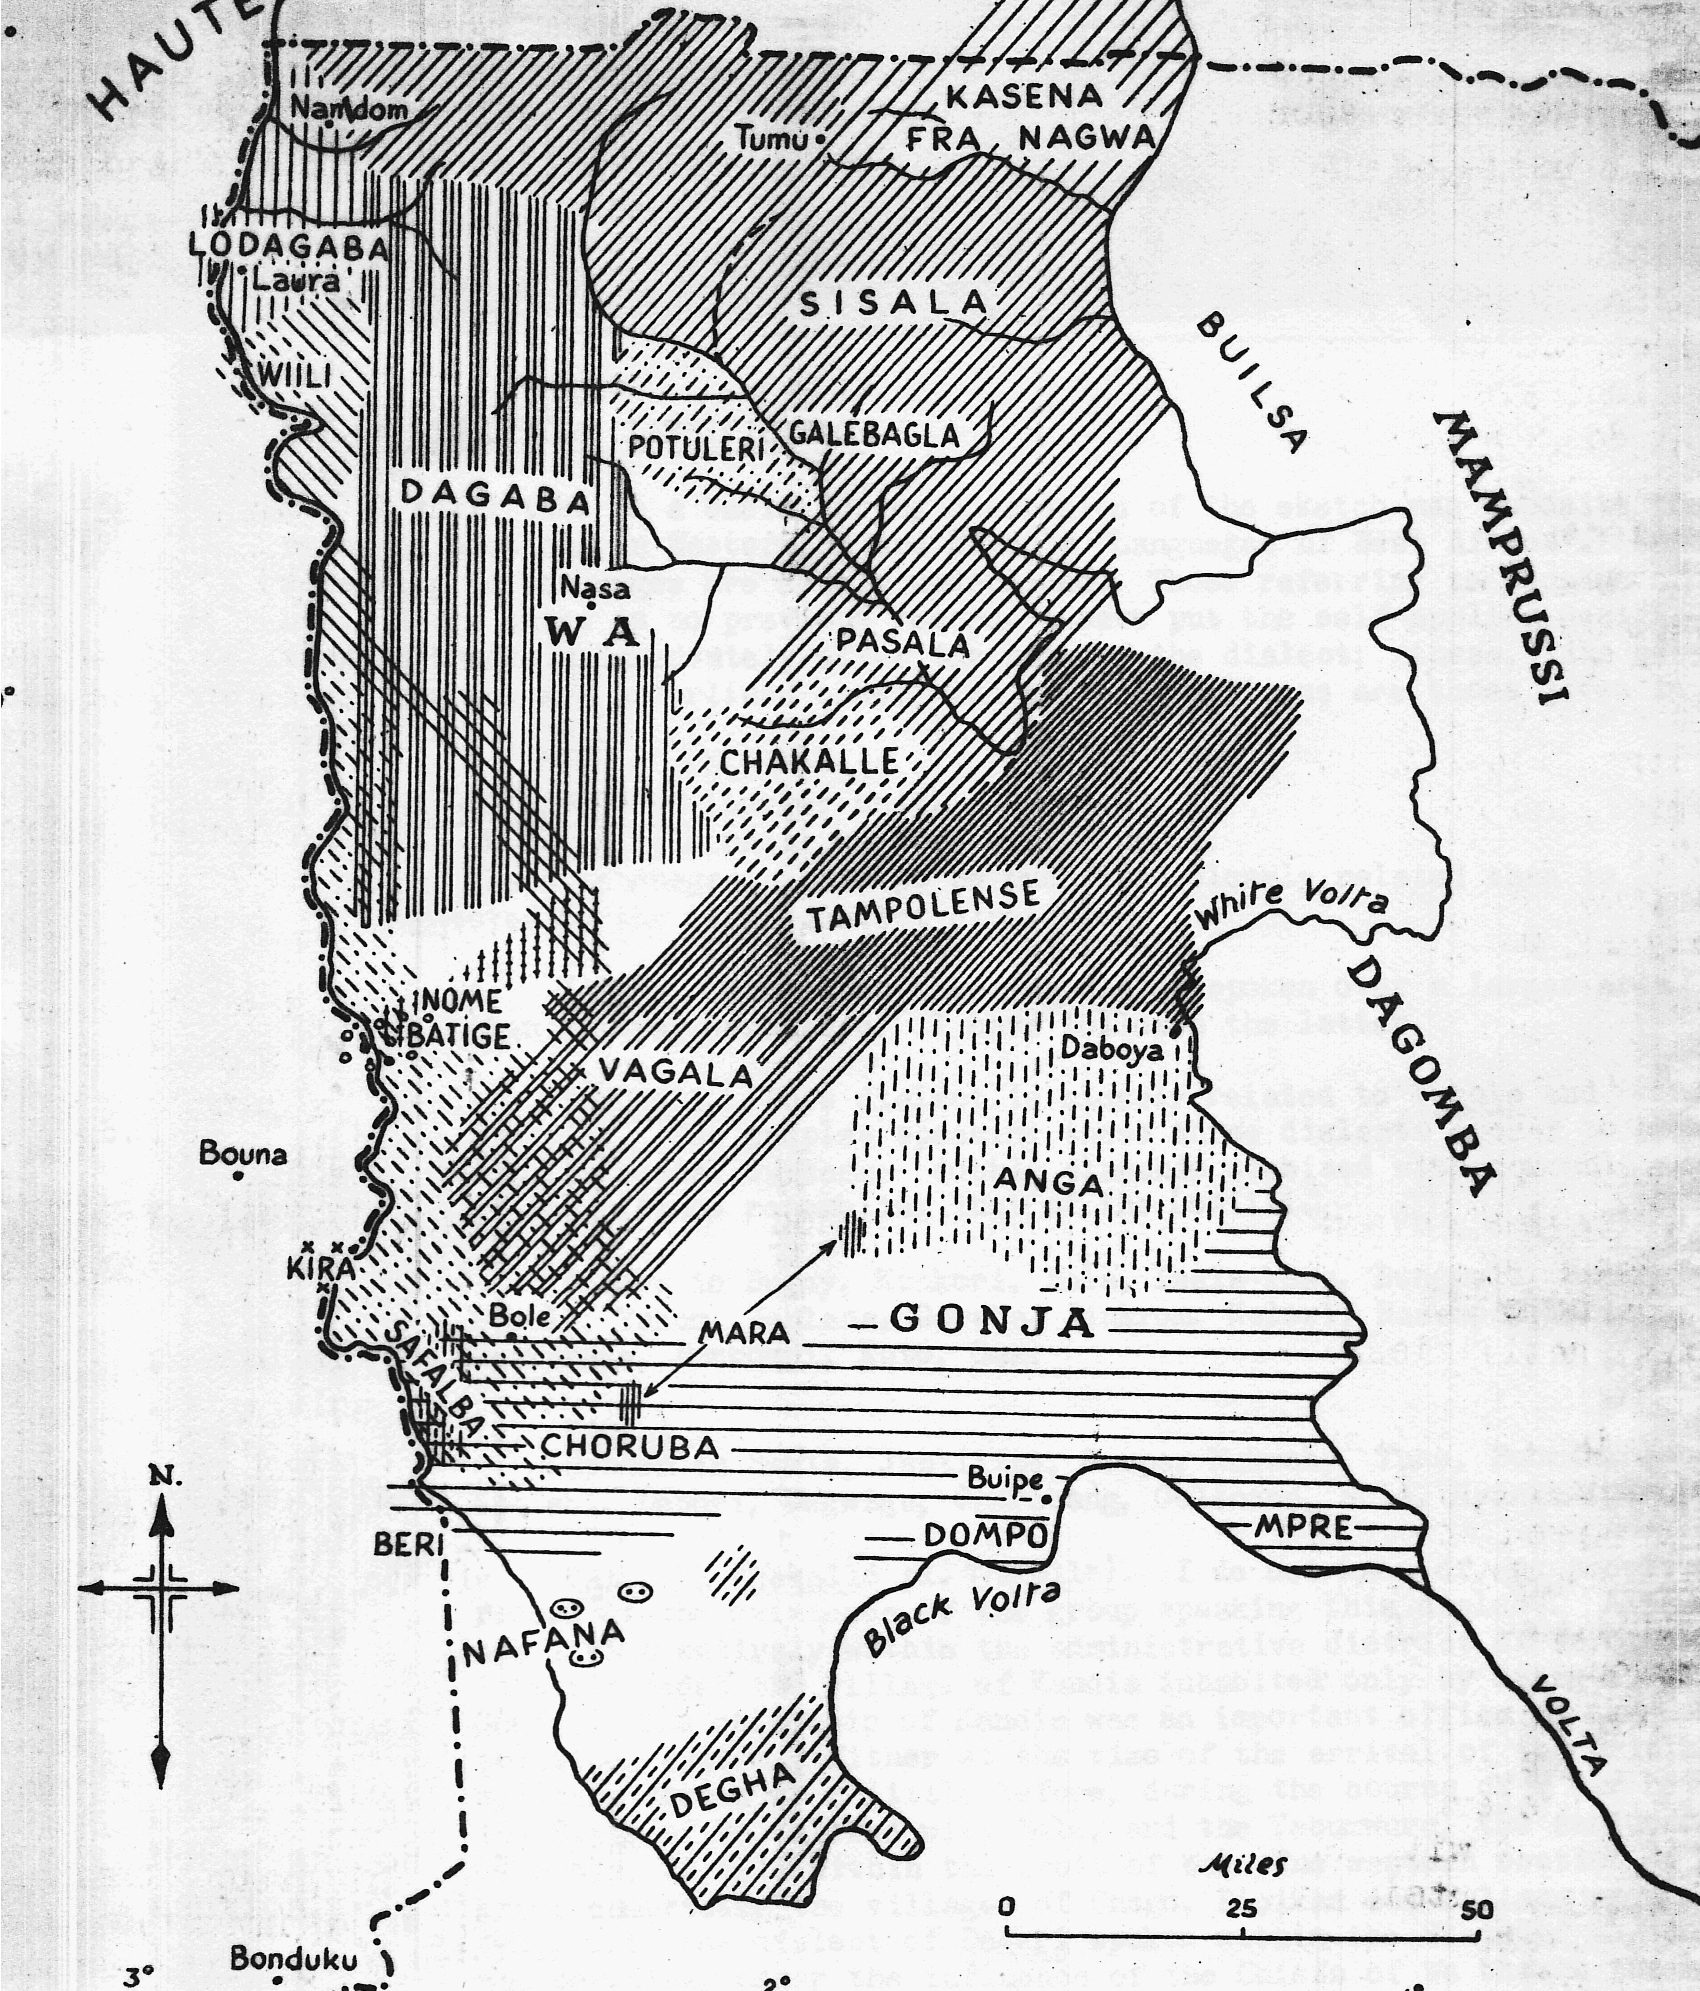
\includegraphics[width=8cm,height=10cm]{Graphic/Maps/Goody54.jpeg}
  \caption[Tribes of the Northern Territories. Source: \cite{Good54}]{The
tribes of the Northern Territories of the Gold Coast west of the White Volta
Source: \citet[2]{Good54} (Modification {\it JAB})
\label{fig:Goody54-map}}
\end{figure}


What I was told about the area is that the people living in the villages
known as
{\S wàwà} (formerly Saala), {\S ɲã́ŋɛ̃̀},\footnote{Nyanga ({\F ɲã́ŋɛ̃̀})  was
the first Gonja capital \cite[121]{Wilk89}.} {\S bùgè}, {\S gbàntàlà},  {\S
káú} (formerly Holumunii), {\S gbɔŋ} and {\S kɔ́nkɔ́rɛ̀} were expelled from the
park some time  in the  sixties. These were probably either Tampulma
or Vagala settlements which had relations, either family ties or common
shrines, 
with the Chakali population of the north. Today, the park visitors  are
told that vestiges of Zabarima raids can be found in the park. Most of the
vestiges are in fact  the villages whose inhabitants were forced to move by the
 government. The population  disperse in all
directions; some went southwest
to villages like Jentilpe, Tuna or Sawla, some went south to Damongo, some
others went east to Daboya or Bowena.  The inhabitants of a Tampulma village
named {\S gbuŋwalɛ} were expelled  in 1964.\footnote{Reported by Mr. Dɔga, an
elder of Ducie's {\F gbuŋwalɛ}, eye-witness of the exile to Ducie.} Some  went
to Ducie, some  to Gurumbele, while some others went to Jentilpe
and other villages in Vagala land.  Today {\S gbuŋwalɛ} can refer to three
locations in a confined area;  the name of a  section in  Ducie inhabited by
Tampulma
migrants,  the original deserted village (25 km from Ducie), or  a ranger camp
belonging to the Mole national park named after the original village. 


Without going  into detail about the park’s history, the point made is that 
the creation of the park restructured the livelihood and the social network of
Chakali altogether. First,  the loss of habitat had a significant impact on
hunting activities and, consequently, their diet. Secondly,  instead of engaging
in their established social network in the south with Grusi speaking groups,
they developed contacts towards the  west, which features Islam as
religion, Waali and
Bulengi as languages (see section \ref{sec:SOC-bulengi}) and centralization as a
mode of administration. The south area was
more or less similar to  traditional Chakali: {\S sɪgmaa} and totemism as
religion (see section \ref{sec:SOC-religion}), Southwestern Grusi as language
type and acephalous administration. 
For the Chakali, the consequence of building relations with the west are
apparent: the fast growth of Islam, the new socio-economic relations
entertained
with the Waala and the view held by modern authorities that acephalous
administration is inefficient.


\subsubsection{Religion}
\label{sec:SOC-religion}

The Chakali name for God is {\S kùósò} (< {\S kùórù wʊ̀sá} `chief god').
A personal god (or a small god, or a divinity)  is called a {\S vʊ́g}.
Individuals make their own small gods, and offer sacrifices to them, believing
that their  god has been serving
them.
Famous shrines of the area are {\S safo kala} in Bulenga,\footnote{We were told
that {\F safo kala} originates from (former) {\F gbuŋwalɛ}.} {\S  dabaŋtʊlʊgʊ}
in Gurumbele and {\S kʊɔlɪɪ} in Sogla. At these shrines, people come with
requests, and they themselves decide what they will promise to give the shrine
later if their requests are granted. The shrines also ensure the local
population
protection against enemies and witches,  good climate,   and peace in the
community. Divinations are done by a {\S
vʊ̀vʊ̀tá}, i.e. a `diviner' or `soothsayer'.  Fire, stick, sand and
cowrie/coins
divinations are still practiced, although I only witnessed the stick
divination. Today at least one soothsayer  can
be found in each village. 

The cult of {\S sɪgmaa}  masks and the related initiation
society is a distinguishing characteristic of some of the Grusi tribes of the
area. Today, the
masks are only displayed and worn during  funerals.  All
Chakali, at least in Ducie and Gurumbele,  respect the customs of {\S sigmaa}.
In other villages,  it seems to depend on the religious orientation of the
elders. I suspect that it is respected, and feared, across Chakali. The
initiation
society is still very active, and members of non-Grusi
communities  can join as well: Gonja, Waala, 
Dagara and  Akan are  recorded  \citep{Brin09b}.  At the
practical level, it is dictated by the customs of {\S sigmaa} that  an
uninitiated individual cannot attend nor see a funeral ceremony. At a more
abstract level,  the rite, through a ritual  song language,  allows
for the
(re)transmission of knowledge  required to be an accomplished  
individual.  It basically teaches the practices underpinning {\S
sigmaa} and  cultural identity.  For instance, the message of a song may contain
examples
of good and bad behavior, while other songs consist of  an introduction to  the
origin of {\S sigmaa}, the identification of important spirits, etc. The point
is that these messages are not specifically targeted at Chakali, but  also  at
Tampulma, Vagala, (some) Sisaala, etc.   or,  in other words, at those who
include  {\S
sigmaa} in their religious customs.  The Waala and Dagaara in particular, being
Muslim, Christian or Tradionalist and  do not practice  the customs of  {\S
sigmaa},
believe
that the initiation rite provides  lifetime protection against witchcraft. This
spiritual armor has a valuable and beneficial use  especially in this area
where witchcraft is a genuine source of fear. The cult has a large repertoire of
traditional medicines, involves magic and accepts the supernatural. The Chakali,
Tampulma and Vagala are known in the region to be among the last practitioners
of
these remnants of
traditional beliefs, which were certainly diverse and  widespread in the
region
and in  West Africa in general. The cult is mentioned in
\citet[5-6, 56-58]{Brav74}, \citet[95-96]{Doug66} and \cite{Popp93}.


Totemism is an integral part of the traditional
religion.\footnote{It was suggested to me to avoid the old-fashioned term
{\it totemism} and change it to `food restrictions', `animal worship' or
`taboos'. I do not fully understand the concept(s) neither in Chakali (culture)
or  the field of anthropology, but  to me food restrictions, animal/insect
worship and taboos are different aspects of Chakali traditional belief,  so I
considered totemism to be a suitable (and unitary) term.} Totem animals
(or
insects) vary from clan to clan and shrine to shrine, probably due to their
specific historical significance. Each descent group has a totem which the
members cannot kill or eat. Table \ref{SOC-danta} gathers information originally
collected on food consumption taboos among men and gives a rough idea of  the dietary prohibitions an
individual  must observe.  The columns present in order an
individual male,  his village and section, his  {\S dántà} `clan appellation',
 and finally his inherited consumption taboo.\footnote{It may be that the
inherited consumption taboo is confused with one's {\F tɔma}, which is similar
but different from a {\F wɔsɪtʃii}. It is unfortunate that \cite{Ratt32a,
Ratt32b} are the only documents  discussing totemism, avoidances and clan names
in Sisaala, Vagala and Tampulma groups. It is surely the most promising way to
study human history in the region.}



\begin{table}[htb]


\centering
\begin{tabular}{lp{4cm}lp{4cm}}
\Hline
I.D.  & Village-Section & {\it Danta} & Inher. Taboo\\ \hline
MAN &Gurumbele-zaban & {\S íjàà} & {\S bʊɔmanɪɪ} `leopard' \\%Manwe naa
AMO &Gurumbele-zaban & {\S íkò}  & {\S kɔnsɪaŋ} `red pigeon', {\S ɔnsɪaŋ}
`type of
mouse' \\%enter in dict%Amoa
ZIE &Sogla-ɲãdʊɔlabanɪɪ & {\S íkò}  & {\S kɔnsɪaŋ} `red pigeon' \\%Zien
AMA & Motigu-wasɪkʊlʊbanɪɪ & {\S íkò}  & {\S òntòléè} `type of mouse' \\
DOU& Motigu-wasɪlɛɛlabanɪɪ & {\S íkò}  & {\S òntòléè} `type of mouse' \\
KUO  &Gurumbele-gurumian & {\S ísì} & {\S ger} `lizard', {\S bãã}
`type of lizard'\\
MAA & Sogla-tindambanɪɪ & {\S ísì} &{\S bãã} `type of lizard' \\
SAL& Sogla- ɲãdʊɔlabanɪɪ & {\S ɪ́wɛ̀} &{\S bʊɔmanɪɪ} `leopard',  {\S ɲʊg}
`crocodile'\\ %stranger
ABS & Tuosa-wɔsɪwɛɛ & {\S ɪ́wɛ̀} &{\S bʊɔmanɪɪ} `leopard',  {\S kɔnsɪaŋ}
`red
pigeon'\\ %what are the sections of tuosa
BAK& Gurumbele-zaban & {\S ɪ́tʃà} &{\S ãã} `bushbuck'\\
TOM & Ducie-lobanɪɪ & {\S ɪ́tʃà} &{\S ãã} `bushbuck'\\
KAN & Ducie-kuorubanɪɪ & {\S ɪ́tʃà} &{\S ãã} `bushbuck'\\
HAK& Gurumbele-zaban & {\S ɪ́tò} &{\S nɪɪɲuugbaŋgbulii} `type of insect'\\
KAS& Motigu-wɔsɪlɛɛlabanɪɪ & {\S ɪ́lɛ̀} &{\S dʊ́kpénì} `type of snake'\\%kasim

\Hline



\end{tabular}
\caption[Information on some clans and taboos]{Information on
 clans,  taboos and  {\M danta}. I.D.= male individual, {\M danta} =
 expression derived from a clan affiliation, Inher. taboo =  inherited taboo. 
\label{SOC-danta}}
\end{table}


Taboos are either inherited or acquired. They usually involve the
interdiction of eating a certain living species or performing certain actions. A
taboo   inherited by paternal lineage is a {\S
wɔ̀sɪ̀tʃìí}: a new born has
automatically  his father's inherited taboos. An acquired taboo may be gained at
a shrine. For instance, when one becomes `a member of' the Sogla shrine
{\S kʊɔlɪɪ},  it is forbidden for the person to eat dog meat.  %what was my duongsoi
 A person’s inherent taboo seems to be intimately
related to
his or her {\S danta}, which is an appellation identifying membership to a
certain
clan and  can also be used in greetings.\footnote{One consultant, A. B. Sakara,
claims 
that all Chakali taboo {\F kɔnsɪaŋ}
`red pigeon'  ({\it Streptopelia
senegalensis}). In \citet[517-520]{Ratt32b},
 the avoidance of red
pigeon was found
among the clans of Vagala and Tampulma he visited.}    Women have more
restrictions on the consumption of some
species, usually due to the effect they have on newborn babies 
(e.g. reptiles and snakes
cause
deformation, hyenas cause sores, etc.). These are neither inherited or acquired
taboos as discussed above,  but may be seen to
represent preventive medicine knowledge.

%{\S ɲaŋgbala}, the current priest of
%the Sogla shrine {\S kʊɔlɪɪ},


Christianity is practiced by some individuals: the church services are usually
held in Ducie. The Catholic Church and  the Evangelical Church of Ghana are
present.\footnote{Information given by Pastor Alex Kipo (Tuosa, Jang, Ducie) and
Mark Zoonaa (Motigu).} Islam has been gaining many more followers than 
Christianity. Since my first visit in 2007,  Ducie has a new mosque and several
new praying grounds, Gurumbele has built a new praying ground, and several
Muslim
youth groups have emerged all over Chakali.  This development is a
source of
concern for the preservation of {\S sigmaa} customs,  which  continuously
involves training drummers and dancers. Some people maintain that  modern
religions do not allow their believers to wear the  {\S sigmaa} costume.
Despite the presence of Christianity and
Islam, the practices of   traditional religion are carried out by some
Christians and Muslims, especially at the funerals. Overall the practice of
modern
religions is syncretic in nature. 


%%%%%%%%%%%%%%%%%











% The  people of the Upper West region speak Oti-volta languages,  such as
% Buli, Kasem, Birifor, Kantosi,  Waali and Dagara, or Grusi languages, such as 
% Western
% Sissala, Tumulung Sissala, Pasaal,  Sissala, Tampulma, Vagala and
% Chakali\footnote{The three letter iso code is from \cite{}}. English is the
%main
% language spoken in educational and governmental institution. The Fula language
% is found in pockets spread across the region.



\section{Linguistic vitality and diversity}
\label{sec:SOC-unesco}


\subsection{Previous sociolinguistic surveys of the Chakali language area}
\label{sec:SOC-gil-socio}

In the last 40 years, two sociological surveys have been conducted in Chakali.
In 1974, the Ghana Institute for Linguistics (GIL) investigated the need for
Chakali
language development \citep{Reim75}.\footnote{This document  listed as {\it
Reimer,
Jean and Regina Blass. 1975. Chakali survey report. GILLBT. unpublished.}   in
\cite{Tomp02}  could not be found
at the GILLBT headquarters in Tamale, nor obtained from one of its authors,
Regina
Blass.} The authors
of the report attested high Waali comprehension in the two Chakali villages
visited. Since written material already existed in Waali, the report concluded
that future development should be linked to Waali literacy effort
because Waali written material was assessed comprehensible in their
survey. A follow-up survey was carried out in 1995 and published in  
\cite{Tomp02}. Commenting on the 1974 survey, \citeauthor{Tomp02} concluded 
that
(i) twenty
subjects in two villages is not enough to demonstrate L2 comprehension (i.e. of
Waali), (ii) understanding Waali material does not imply speaking Waali,
therefore the degree of  bilingualism of the Chakali people  cannot be
demonstrated (i.e. \cite{Reim75} refers to bilingualism), and (iii) in word
lists, the presence of Waali terms does not indicate bilingualism; borrowing
 is a more probable explanation. The authors of the follow up 1995 survey
reiterate that ``the purpose of the survey was to help
administrators [of GILLBT] decide whether there is a need for Chakali
language development or whether these communities should be linked to Waali
literacy efforts''  \citep[3]{Tomp02}. 

According to them, Chakali language development needs were to be determined by:
(i) assessing Waali
comprehension, first from the reported data and later from tested data if
necessary, (ii) assessing the use of Chakali and Waali in various domains, to
determine whether there were indications of language shift toward Waali, (iii)
assessing language attitudes related to potential community involvement in
Chakali language development, (iv) gathering information on population,
education
levels, literacy, religious environment and language contact with Waali
speakers, (v) assessing Dagaare comprehension and Dagaare use, since Dagaare is
the official regional language, and  (vi) assessing Vagala
comprehension, as
Vagala
is closely related to Chakali. The survey was carried out in Katua, Motigu and
Ducie. 

Among many other revealing figures, their results show that all 37 individuals
interviewed (i.e. 100\%) in the three villages report the ability to speak and
understand Waali. While 24\% can understand Dagaare, only 8\% can speak it. And
while 44\% claim to understand Vagala,  only 3\% report the ability to speak
it. The village of Ducie  reports  least use of Waali in public domains, while
Katua reports most use of Waali at home. Overall, Waali is used more in
Katua and Motigu than in Ducie, and females more than males report Waali in
daily use.

The information provided in \cite{Tomp02} is very similar to what I
observed. Although I did not go through similar  questionnaires, their
conclusion clearly reveals that  inhabitants of Ducie, Motigu and Katua do speak
and understand Waali. GILLBT administrators therefore decided that ``Chakali
language development would not be pursued'' because ``Waali comprehension and
use was high enough and its use was extensive enough for the use of Waali
written materials'' \cite[23]{Tomp02}.

%Dakubu
%Awdoba: People of northern Ghana. Socio-Method-Intro folder
% \footnote{Waali is ``a dialect of
% Dagaare little different from that spoken in Kaleo and the other Dagaaba
% villages of the district''\citep[][pg~16]{Wilk89}}
% \cite{Lewi05} uses the factors and evaluated them...

\subsection{The Unesco Survey}
\label{sec:SOC-unesco}

In \citet[2]{Reco03}, it is  stated that  ``a language is endangered when it is
on
a path toward extinction''  and  ``in danger when its speakers cease to use
it''.  To my knowledge, statements qualifying Chakali as `endangered'  appear
in \cite{Daku05} where  the language ``can indeed be classed as an endangered
language in the medium term'',  and in \cite{Awed06},  which asserts that  ``the
language is almost dying out''.\footnote{\cite{Awed06} also writes that
``Chakali live in communities that acknowledge Gonja overrule and usually have a
resident Gonja Chief living among them''. This information is erroneous.
The Kandia  jurisdiction of Gonja was transfered to Wa approximately  a hundred
years ago. Also, as mentioned in section \ref{sec:INT-lit-rev}, Prof. M. E. K.
Dakubu gathered information from a native of Jayiri whose mother was a Chakali
speaker, whereas the statement of Prof. Awedoba is not substantiated.}

% \citet[33]{Good54}, quoted in section \ref{sec:INT-lit-rev}, writes that the
% Chakali  ``{\it seem to have been}'' under the Gonja chief of Kandia, but that
% the whole Chakali remains to be confirmed by Chakali and Gonja history.

To assess the current situation in Chakali,  the questionnaire developed
in \cite{Reco03} is used. This   document is  ``designed to assist language
communities,
linguists, educators and administrators (including local and national
governments and international organizations) in finding ways to enhance the
vitality of threatened languages.''   It  provides  nine factors that
both  identify imperative needs and give the researchers a broad idea of the
state of endangerment of a language.  The authors acknowledge that no single
factor alone can be used to assess a language's vitality or its need for
documentation. The integration of the nine factors is ranked on a continuum from
stability to extinction.  In this section, I evaluate  each factor defined in
the framework. These are (i) intergenerational language transmission,
(ii)
absolute number of speakers, (iii) proportion of speakers within the total
population, (iv) trends in existing language domains, (v) response to new
domains and media,  (vi) materials for language education and literacy,
(vii) governmental and institutional language attitudes and policies, (viii)
community
members’ attitudes toward their own language, and (ix) amount and quality of
documentation.   In section
\ref{sec:SOC-overall-vitality}, the factors are
evaluated either on a scale or  provided with absolute numbers.  It is
important to mention that information for certain villages only is available,
more limited 
for some than others. In this section,  the villages
appearing in  figure \ref{fig:INT-cliland} of chapter
\ref{sec:INT-introduction} are discussed, e.g. Tiisa, Tuosa, Sogla, Motigu,
Ducie, Katua and Gurumbele. The
villages   Bulenga, Chagu, Chasia, Bisikan, Kandia,
Dupari and Gilan are not included.  The main reason is that various
individuals told me not to look for the Chakali language in these
villages.\footnote{I did not visit Chasia,  but it is a village in need of
a 
sociolinguistic survey. Its contact with and proximity to the
Vagala on the one hand, and  with Jayiri (Waali-Bulengi) on
the other hand  makes the village an interesting site.} Besides, everyone 
seemed
to agree that Ducie and Gurumbele are
the places where one can hear Chakali in its `uncorrupted' form, even though
Sogla is claimed to be the first Chakali settlement. Needless to say, the
outcome
is  at best qualitative and must be regarded as provisional as I did not carry
out a systematic survey for each
factor.\footnote{In discussing the nine factors below, a word in italics
reproduces an evaluative term used in
\cite{Reco03} and bears the sense found therein.} 




\subsubsection{Factor 1: Intergenerational language transmission}
\label{sec:SOC-Factor1}

It is fair to state that the children in Ducie and Gurumbele all speak
Chakali, and that in Motigu and Katua the great majority of children  speak the
language.  In Katua,  there are more women from Pasaale
speaking communities who are married to men of the village than anywhere else,
and family members of the chief who speak Waali also live in the village. For
Sogla, Tiisa, and Tuosa, children may be said  not to speak Chakali but a
minority may be
able to undertstand their parents or grandparents when they speak.  In Motigu and Katua, Chakali is
used by a majority, whereas in
Sogla, Tiisa and Tuosa the language is used by the parental and grandparental
generation only. The language is therefore {\it definitively endangered} in the
latter
three villages as it is no longer being  learned as  mother tongue by
children in the home.  I was told  Waali is the language which has taken
over.   With respect to   inter-ethnic alliances, it is
possible that
in any village, 
mothers want to equip their children with  their own native language (e.g. 
Dagaare, Waali, Vagala, Tampulma or Pasaale), but a child's usage of the
language
would then be restricted to  specific social domains (i.e. such as at home
with the mother and when maternal family members come to visit).  

% A 
% factor which places Ducie apart is that it is the only village without Lodagaa
% settlers. 


\clearpage

\begin{table}[htb]


\centering
\begin{Itabular}{lllll}
\Hline
Village-Section & Individual & Household & House & Individ./Hshold.\\[1ex]
\hline
\multicolumn{4}{l}{\it Ducie}\\[1ex] \hline

gbʊŋwalɛ &292 & 50 & 42&5.8 \\
zɪŋbanɪɪ&106& 18 & 17&5.9\\
paŋbanɪɪ&155 & 31 & 23&5\\
lobanɪɪ&272 & 53 & 45&5.1\\
kuorubanɪɪ/gatɪgɛ & 563 & 97 &83&5.8\\
fulani&31 & 5 & 2&6.2\\
\hline
\textsc{total}& 1419 & 254 & 212& 5.6\\[1ex]\hline

\multicolumn{4}{l}{\it Gurumbele}\\[1ex] \hline


 zaban& 301 & 43 & 38&7\\
gurumian& 252 & 45 & 27&5.6 \\
belekani& 119 & 17 &17&7 \\
fulani& 11 & 2 & 2&5.5\\
\hline
\textsc{total}& 683 & 107 & 84&6.3\\[1ex]\hline


\multicolumn{4}{l}{\it Motigu}\\[1ex] \hline

wasɪkʊlʊ& 409 & 71 & 68& 5.7 \\
wasɪlɛɛla& 233 & 37 & 36& 6.3\\
dagaaba&111 & 22 & 19&5 \\
fulani&26  & 3 & 3& 8.6\\
\hline
\textsc{total}& 779 & 133 & 126&5.8 \\[1ex] \hline

\multicolumn{4}{l}{\it Katua}\\[1ex] \hline

jarabalɪɛ       &168    &27     &9 &6.2\\
dantobalɪɛ	&93 	& 13 	& 5& 7.2  \\
koŋkorɪɛ	&32     &5      &2  & 6.4\\
kuruŋkatʊɔlɪɛ	& 66	&10	&5 &6.6\\
buleŋi	        & 42 	& 7 	& 2 &6\\
dagaaba         &147	&23	&20 &6.3\\
chief palace	& 6 	& 1 	& 1  &6 \\
fulani 	        &99	&4	&	4 &24.75 \\
\hline

\textsc{total} &653 &90& 48 &  7.2\\[1ex]\hline
\textsc{grand total} & 3534&584&470& 6  \\[1ex]\Hline
\end{Itabular}
\caption{Populations of Ducie, Gurumbele, Motigu and Katua (author's field survey, January 2008)
\label{tab:pop-DBMK}}

\end{table} 

\clearpage


\subsubsection{Factor 2:  Absolute number of speakers}
\label{sec:SOC-Factor2}

 
 \citet[17]{Wilk89} reports that the
population of  Ducie was 350 inhabitants in 1948,  and 529 inhabitants in 1960. 
\citet[144]{Nade89} classifies Chakali as a medium-small language (i.e. 5000-50
000 speakers) 
and
\cite{Tomp02}
estimates it at  5,000 speakers. \cite{Daku05} writes that ``[t]he 2000 census
(...) suggests far fewer [than 5,000]''.  The
question to ask is what was meant by `Chakali' when these censuses and surveys
were
carried out?  For instance, if one adopts the `Chakali' of \cite{Daan94},  the
populations
of  13 villages need to be added up.  

%\cite{Tomp02} is based on Boateng 1984



My estimate of the absolute number of speakers  uses a population survey we
carried out in
2008 in the four villages Motigu, Ducie, Gurumbele and Katua.\footnote{For the
survey in Katua (2008-03-11),  I was  assisted by Idriss Haruna and Dakurah
Francis. For the three other villages, Jamila Osman and Mr. Abraham assisted
me (2008-01-15).} Table \ref{tab:pop-DBMK} gives the village and section names,
the number of individuals, households and  houses, and finally, in the last
column,  the percentage of households per house.\footnote{See footnote
\ref{ft:hshold} for  information on how we defined household in the survey.}
From the grand total appearing in the second column of table
\ref{tab:pop-DBMK} (i.e. 3534)
is subtracted the number associated with Fulani, Lodagaa and Waala settlers
(i.e. 550). To the number of speakers in the four villages (i.e. 2984) is
added a generous 500 representing an approximate number of speakers from the
parental and 
grandparental generations in Sogla, Tiisa and Tuosa and speakers in the
diaspora
(Bulenga, Wa, Accra, gold miners in Brong-Ahafo region,
etc.). Therefore,  the estimate of the absolute
number of
Chakali  speakers is 3484. Future work  may want to look closer at
Chakali as a second language and its level of proficiency in the villages of
the area and in
the diaspora, especially among children living outside Chakali land.\footnote{I
do not discard the population of Ducie's section
{\F gbʊŋwalɛ}. Even though they speak a variety of Tampulma very close to
Chakali, the
majority of  Tampulma children and young adults converse using Chakali outside
their section. For Tiisa and Tuosa I expect  the percentage of Chakali speakers
to be similar to Sogla. The table below presents the results of a population
survey I carried out in Sogla in April 2010. 

\begin{center}

\begin{tabular}{lllll}
\hline
Village-Section & Individual & Household & House & Individ./Hshold.\\[1ex]
\hline
\multicolumn{4}{l}{\it Sogla}\\[1ex] \hline

 tindambanɪɪ      &	143&	31&	 22&4.6 \\
     ɲãdʊɔlabanɪɪ    &	192&	46&	39 &4.2 \\
      busalabanɪɪ &	75&	16&	9 & 4.6\\
     dagaabajirii   &76	&14	&	12 &5.4 \\
\hline

\textsc{total} &486 &107&  82& 4.7 \\[1ex]\hline
\end{tabular}
\end{center}


 About a fifth of the
population (i.e. 96), mostly individuals of {\F tindambanɪɪ}, told
me  they understand Chakali and that some of them speak it at home. The rest of
the
population speaks Waali or Dagaare.}  



\subsubsection{ Factor 3: Proportion of speakers within the total population}
\label{sec:SOC-Factor3}

My estimate  of the population of Chakali speakers (i.e. 3484) in section
\ref{sec:SOC-Factor2} makes  0.5\% of the Upper West region's total population, 
and  0.01\% of the Ghanaian population.\footnote{The population of the Upper
West (i.e. 573,860) is taken from \cite{GSS00} with an annual growth rate of
1.7\%.  The Ghanaian population (i.e. 23,350,927) is taken from the World Bank,
World Development Indicators ({\it www.google.com/publicdata}. Accessed on July
26, 2010).} With these numbers, Chakali is arguably the smallest Southwestern
Grusi
 language and one of the smallest languages in
Ghana in terms of L1 speakers \citep{Lewi09}. These numbers are quite different from
the  numbers provided by the Wa East district. The District Assembly in
Funsi
suggests that Chakali make up  19\% of the Wa East district, which is estimated
at  66,358 inhabitants \citep{GSS00},  i.e. approximately 12,000 speakers.   Here again, the interwoven  concepts of
land, ethnicity and language seem to have affected the result. 


\citet[9]{Reco03} maintains that the number of speakers of an ancestral language
in relation to the total population of an ethno-linguistic group is a
significant indicator of language vitality. If we believe the elders I talked
to and accept that the villages  Sogla, Tiisa, Tuosa, Katua and Motigu were at 
a certain point in time monolingual Chakali, then  today's  situation is that
only a {\it minority} of the Chakali people speak the language. 

\subsubsection{Factor 4: Trends in existing language domains}
\label{sec:SOC-Factor4}

The languages of formal education are common to all villages. The current
situation in Ghana is that English is the main language of instruction, and each
region has a local language with
an established orthography recognized for education purposes by the Ministry of
Education.\footnote{Materials are available in
ten of the 79 Ghanaian languages \citep{Lewi09}, i.e. Akan, Ewe, Ga, Dangme,
Nzema, Dagaare, Gonja, Gurenne, Kasem and Dagbani. The total number of Ghanaian
languages varies across sources. } In Chakali schools, the 
indigenous Ghanaian language being taught is Dagaare. Teachers in Ducie and
Gurumbele, half of them from Wa or Lodaaga communities,  told me they have hard
time teaching this subject, and added that it is often dropped altogether
towards the end of the school year in order to focus on the core and more urgent
subjects for the final exams. Compared to other places in Ghana, the schools in
the villages of the Chakali area have probably an average success rate in terms
of government education. The infrastructure is there; there are also teachers
and
sometimes the required material. Only Sogla has no school but this is just a
question of time.\footnote{The building was completed in 2010.  Most
school children of Sogla attend school in Tuosa or Motigu , or move to 
relatives in a
village where there is a school.}  The schools, the teachers and the pupils all
look very good
on a report or on an afternoon visit. When it comes to the goal of the
infrastructure, i.e.  education, it is hard to tell whether the situation can be
considered successful. In 2008, in Ducie school,  I often took over for
missing teachers, teaching mathematics in  a primary 6 class using English as
the
medium of instruction.  I saw harsh caning, some Junior Secondary School
students (12-16 years old) who could simply not read, hard labor work (farming,
food making, digging), etc. Another observation is that classrooms are deprived
 of dialogue. Pupils are afraid and confused, and whenever a child speaks, it
is rote repetition usually disconnected from his/her understanding. The former
headmaster of Ducie school had revised the local language policy  in 2008;
instead of being caned for speaking Chakali in school (or in school area
altogether), a fine had to be paid, an amount about the same as the wage of a
woman's work collecting and selling wood in a day. Usually the teachers
 collect the money. Obviously,  there is  active repression of
Chakali, both by the school management and the imposed national curriculum. In
my  view,  the school is the first social and educational institution a Chakali
child meets in life  which depreciates and devalues his/her language.


Another domain where Chakali was and still is  suffering from active repression
is the domain of  external relations.  Leaving aside the
historical details of the original Chakali-Waala alliance, the imposition and
enstoolment of Waala chiefs by the Colonial Administration in Chakali villages
upset the pre-colonial, balanced cooperation between the Chakali and the Waala.
According to \citet[]{Daan94}, strangers taking decisions in a village is
unprecedented in Chakali history. In colonial times,
chiefs were known for their abuse of  power. In consequence, Chakali
inhabitants
tried their best to avoid  a case leaving the village and being reported
to the native courts set up by the colonial administration  in Bulenga,   Busa
or Wa.  It is certainly around
that time (i.e. approximately fifty to seventy years ago), that Chakali speakers started
to suppress their language in favor of Waali. This may have been out of cautiousness, in order to avoiding misunderstandings and conflicts with their chiefs. However, such a language shift must have been first
limited to administrative meetings and further extended to general social
contexts.  
%but hard to delienate the administrative from the social in those social
%organisation


Nowadays, the government of Ghana speaks through an `assembly man' at the
community level.
He/she  is elected at the community level and  represents one community,
or sometimes two,  at the district level.  Even though that person is a local,   he/she is generally educated and does not live
on-site.  The fact that the `assembly men' are rarely in the communities forges dissatisfaction among people. That is why  recently local teachers, who are
literate and reside in the
village,  are elected. Too often I have witnessed governmental officials visiting Ducie while
the `assembly man' was absent.\footnote{A good explanation is that the villages
under
discussion are not covered by the current mobile phone networks. Local
 assembly men are thus always taken by surprise when representatives of the  District Assembly pay
a
visit to the villages.} The solution is then to select someone who speaks a
common language with the visitors in order to have their message transmitted.
English, Waali and Akan are frequently used on such  occasions. Because the area
is still very remote, other governmental services are not found in Chakali,
except for a clinic in Ducie established in 2002. The personnel speak English
and Waali. 


%parity must be understood as a stable balance in domain use for individual
%speakers 
%Saving languages: an introduction to language revitalization
% By Lenore A. Grenoble, Lindsay J. Whaley

In summary, the situation in Ducie and Gurumbele is one of {\it multilingual
parity} since English and Waali are used as the primary languages in most
official domains.  Speakers do experience active repression of Chakali in
domains like
education and modern administration. Chakali is integral to a number of public
domains, especially traditional religious institutions, local stores, and
  where members of the community socialize. In Ducie, Gurumbele,
Motigu and Katua, the coexistence of  Waali and Chakali  is a good example of
diglossia, which was already established in \cite{Tomp02},  whereby Chakali  is
used in  informal and home contexts,  and Waali and English are used in official
and
public contexts. For Sogla, Tiisa and Tuosa,  diglossia is representative of
only a  minority of the overall population.  Nevertheless, the  Chakali language
in Motigu and Katua may be categorized as {\it dwindling}; Waali spoken at home
is reported to be increasing in both villages . Traditional religious and
administrative institutions are fading away. However, while
Waali is spoken and understood by a majority in all the villages,  there are at
most 1-4 individuals per village who can speak and understand English.
Finally,
it is hard to argue at this point on how `prestige' plays a role in the
linguistic choices and  the level of production and comprehension of
English among school children.

\subsubsection{Factor 5: Response to new domains and media}
\label{sec:SOC-Factor5}

Lacking electricity,  most modern media devices   are useless in the 
villages.
Battery operated radio is the only reception device found in the village,
apart from the talking drums which are used to communicate with neighboring
villages.  The first radios in Ducie
were brought by Waala teachers. Today many youths and adults own a
radio. They are mostly
listened to at night or brought along to the farm, especially when one plans
to stay  overnight. The  broadcast languages are  Waali, English and
Dagaare by  Radio Upper West and Radio Progress, both
sending from Wa.  News in Tumulung
Sissala is presented as well by both stations.  In Ducie, these are the two
radio stations which can be taken in, though it is possible to receive Radio
Savannah which transmits from Tamale. The literacy rate is not known, but
apart from the school children, the teachers and a handful of adults who
attended primary school, no one else can read or write in the villages. Books
and
old newspapers are found in school. Chakali is forbidden in school, as
mentioned in section \ref{sec:SOC-Factor4}. Chakali is used to preach by some
Christians, an initiative of Pastor Kippo who himself claims to have been
involved in the Vagala literacy program, but this is the only case I found
where the language is being used in a new domain. Based on these details, I
regard 
Chakali as a language  hardly used in any
new domains (i.e. roughly defined as modern medias and modern religions).


\subsubsection{Factor 6: Materials for language education and literacy}
\label{sec:SOC-Factor6}

Although several studies in recent years have shown that education in the native
language is essential for language vitality, Chakali has not been implemented in
formal education.  Today it is hard to say whether the speakers wish their
language to be written.  Basically, `yes', they do, perhaps only for the status.
Some people I talked to are upset about the fact that all their neighbors have
a
literacy program.\footnote{We suspect they have in mind the GILLBT literacy
programs for Vagala, Tampulma, Pasaale, Sisaala, Hanga and Gonja, and the
Baptist church literacy program for Waali.} My impression  is that
Chakali
literacy
would be first a  source of pride, and second a challenge for formal and
non-formal education. If we accept the claim that literacy is directly linked
with  social and
economic development, then  materials on all topics for 
various ages
and language abilities and people to teach them  are needed, i.e. a language
program
\citep[see][7]{Gren06}. 


Based on these observations,   the language can be said to not have an
orthography nor material.  However, I acknowledge the efforts made by Pastor
Ronaldo who in 2001 designed two illustrated booklets with the intention of
starting a vernacular literacy project. With the agreement of the headmasters, I
 introduced an orthography to some school children in Ducie and Gurumbele. They
all learned it very fast. With Daniel Kanganu, I wrote two short books which
were distributed to the schools in Motigu, Katua, Ducie and Gurumbele (see
appendix on page \pageref{chap:TXT-text}). However, I  cannot claim that ``a
practical
orthography is known to the community'' and that ``some material is being
written''  \citep[12]{Reco03}, since the orthography is not known to the
community as yet and, while
it is true that material has been written, the majority of the speakers are not
`aware' of it. 




\subsubsection{ Factor 7: Governmental and institutional language attitudes
and policies, including official status and use}
\label{sec:SOC-Factor7}

In the government's records, the Chakali people are either ethnically {\it
Waala} or {\it Grussi} / {\it other Grusi} \citep{GSS00, Ghan08}, two
ill-defined concepts (see references on Grusi in section \ref{sec:INT-lit-rev}, 
and \citet[398]{Ratt32b}, \citet[2]{Mano51} and 
\citet[13-17]{Wilk89} for  views on the heterogeneity of  `Waala').  Although
Chakali may be recognized for the first time as one ethnic group in the next
population and housing survey (expected to start in September 26,
2010), there are no efforts being made by the government to recognize the
language and promote it.  The office of formal education favors 
English and Dagaare in the Upper West region. The office of non-formal
education, targeting people within the working age group 15-45, especially
women,  has
made some efforts to teach communities other languages than the official ones,
but Chakali has not been considered.

We saw in the two previous sections  that the government  has explicit policies
in education and that communication with the government (or through any of its
institutions) at the community level is conducted in
Waali, Dagaare, or English. Chakali can arguably be said to  face {\it
active assimilation} since ``the government encourages minority groups to
abandon their own languages by providing education for the minority group
members in the dominant language'' and that ``speaking and/or writing in
non-dominant languages is not encouraged''  \citep[13]{Reco03}.  Chakali
is neither recognized nor protected. 





% However there is hope for the future since Ghana has signed the
% Universal.... the situation and ...(daily graphic. March 18 2006 p.7, February
% 24, 2006 p.7, February 24, 2006 p.24, March 23 2006, p.34)''
% 
% The Universal Declaration of Linguistic
% Rights\footnote{{\it http://www.linguistic-declaration.org/index-gb.htm}
% (Accessed on August 25, 2010)}
% \begin{Quote}
% {\bf Article 24-} All language communities have the right to decide to what
% extent their language is to be present, as a vehicular language and as an
%object
% of study, at all levels of education within their territory: preschool,
%primary,
% secondary, technical and vocational, university, and adult education.
%  \end{Quote}
% 
% \begin{Quote}{\bf Second final disposition} This Declaration recommends and
% promotes the creation of a World Commission on Linguistic Rights, a
% non-official, consultative body made up of representatives of non-governmental
% organizations and organizations working in the field of linguistic law.
% \end{Quote}



\subsubsection{Factor 8:  Community members' attitudes toward their own
language}
\label{sec:SOC-Factor8}

This factor needs considerable attention on the part of the researcher and
reflection on the part of the community investigated \citep[27]{Lewi05}.  I do
not claim to have paid special attention to the community members' attitudes
toward their own language, so it is difficult to evaluate without surveying the
question among the community as a whole. Generally, the people in Ducie and
Gurumbele  praise the attention I have shown to their language and would support
language maintenance initiatives.  Since the great majority also speaks Waali,
the Chakali people are not hindered from economic mobility and integration  into
`mainstream society'. Further, it is not a problem, even for some a source of
pride, for two men to speak Chakali to one another in Wa town.  However, this
attitude is probably recent and due to the decreasing authority of the chiefs.
Adaptation and conversion to the Waala language and lifestyle is not necessary
anymore; the Chakali people come to Wa to trade and go back to their respective
villages. There is no fear of retaliation by dominant Waala. Nevertheless, a
social group which may be highly influenced in terms of attitude toward their
language is the group of Senior Secondary School students leaving the villages
every year for education. When they move to Wa (or Jirapa, Lawra, Nandom, etc.),
they normally become Muslim (or Christian) and  adopt  Waali (or Dagaare).  I
suspect that this group alone considers Chakali to be characterized by qualities
such as backwardness and behind others in `progress' or `development'. This
attitude develops from the prospect of Chakali failing to meet the challenges of
modernity. Rarely do such pupils move back to settle in the villages upon
completion of their  education.

\subsubsection{Factor 9: Amount and quality of documentation}
\label{sec:SOC-Facrto9}

Copies of two booklets were printed and distributed in 2001 by the  Evangelical
Church of Ghana (see sections \ref{sec:INT-lit-rev} and \ref{sec:SOC-Factor6}).
To
my  knowledge, one copy remains. In 2008,  Danial Kanganu and I published two
short stories \citep{Kang07a, Kang07b}. Four copies of each were distributed in
schools. In 2009, I gave one copy of a Chakali-English dictionary to 5
individuals in Ducie and Gurumbele.  The situation may be graded as {\it
inadequate},  and apart from the output of the current project, no phonological
and grammatical sketches, no fragmentary texts, audio and visual recordings 
exist.


\subsection{Score and summary}
\label{sec:SOC-overall-vitality}

The discussion regarding the nine factors suggests a division of the Chakali
villages into three groups  (see figure \ref{tab:estimate-endangerment}). 
Sogla,
Tiisa and Tuosa correspond to the villages where the intergenerational
transmission is ineffective and where Waali is used in formal and informal
domains. They are  the E(ndangered)1 villages. Motigu and Katua correspond to E2
villages. In both villages, I was told that Waali is encroaching on  Chakali in
formal and informal domains. The situation is not alarming since Chakali is
spoken by the majority and  the intergenerational transmission is effective, but
given the average population size of the villages and the recent conversion to
Islam of their youth, it is worth considering that a language shift to Waali may
take place within a short time.  A. B. Sakara and H. S. Daanaa, both born in
Tuosa, told me that Chakali was spoken by everyone in their village when they
were children, i.e. 1950-1960. There  are no signs indicating that the same 
language replacement which took place in Tuosa  cannot take place in Motigu and
Katua. Finally, the E3 villages, Gurumbele and Ducie, show the most effective
intergenerational transmission of the Chakali language. Both villages also
establish local alliances (i.e. marriage, common shrines, one assembly man for
both villages, etc.). Waali is spoken and understood, yet it is usually specific
to formal domains, for instance  official visits conducted by governmental
bodies or  Waala visitors.

\begin{sidewaysfigure}

  \centering
 \begin{Itabular}{p{7cm}p{4cm}p{3.5cm}p{3.5cm}}


 %\begin{tabular}{ll}
\Hline
    Factors & \multicolumn{3}{c}{Measures}\\[1ex]\hline
 &E1&E2&E3\\[1ex]\hline

1. Intergenerational Language Transmission &  {\it severely endangered} 
(2) & {\it unsafe} (4)& {\it safe} (5)\\

2.  Absolute Number of Speakers  &
\multicolumn{3}{c}{[{\it  3484}]}\\ 

3. Proportion of Speakers within the Total Population &
\multicolumn{3}{c}{[{\it severely
endangered}  (2) ]}\\

4.  Trends in Existing Language Domains & {\it highly limited domains}
(2)& {\it dwindling domains} (3)&{\it multilingual parity} (4)\\

5.  Response to New Domains and Media&{\it inactive-minimal} (0-1) & {\it
inactive-minimal}
(0-1)& {\it inactive-minimal} (0-1)\\

6.  Materials for Language Education and Literacy & 
\multicolumn{3}{c}{[{\it no orthography available} (0)]}\\

7. Governmental and Institutional Language Attitudes
and Policies, Including Official Status and Use &
\multicolumn{3}{c}{[{\it active
assimilation} (2) ]}\\


8. Community Members Attitudes toward Their Own Language &-&-&{\it all
members value their language and wish to see it promoted.} (5) 
\\

9.  Amount and Quality of Documentation &
\multicolumn{3}{c}{[{\it undocumented-inadequate} (0-1) ]}\\


\Hline
  \end{Itabular}

 \caption[Estimated degree of endangerment for the E1, E2 and
E3 villages]{Estimated degree of endangerment for the E1 \{Tuosa, Tiisa,
Sogla\}, E2 \{Katua, Motigu\} and
E3 \{Gurumbele, Ducie\}. A value within square brackets  applies to E1, E2 and
E3 villages as a whole}
  \label{tab:estimate-endangerment}

\end{sidewaysfigure}



 \cite{Reco03} proposes that  
the nine factors  should be assigned a score. In the assessment, the score is
either graded on a  0 to 5 scale, or absolute, as for factor 2.   This can be
illustrated  with an example taken from figure
\ref{tab:estimate-endangerment}, which summarizes the vitality and endangerment
of Chakali. For
factor 1, I assign grade 5 to Ducie and
Gurumbele, grade 4 to Motigu and Katua, and grade 2 to Tuosa, Tiisa and Sogla.
 Grade 5 represents a {\it safe} language which is used ``by all ages, from
children up'',  stage 4 represents an {\it unsafe} language which is used ``by
some
children in all domains and all children in limited domains'', and  stage 2
represents a {\it severely endangered} language,  as it is mostly used ``by the
grandparental generation and up'' \cite[8]{Reco03}. 


 Based on  observations,
interviews and a population survey, my estimated degree of
endangerment of Chakali is {\it severely endangered} in  E1 villages, {\it
unsafe/vulnerable} in E2 villages and {\it safe} for at least another generation
in E3 villages. Overall the language may be said to be highly vulnerable.  

%as the number of speakers is relatively low


% Despite the fact that the
% number of speakers is a reliable factor in  evaluating the state of
% endangerment
% of a language, the assessment can not solely rely on this factor. For example,
% if  a language is effectively  pass to younger generation in all domains, the
% language can not be regarded as endangered, regardless of the number of
% speaker.


\section{Discussion}
\label{sec:SOC-discussion}

This chapter concludes with a  brief discussion of  dialectal variations, 
the case of the Bulenga language,  and finally,  some
summarizing thoughts on the language's vitality.





\subsection{Dialectal variations}
\label{sec:dialect}

The people of the villages under discussion are known as the  {\S m̩̀ ŋmá
kàà} `I say so', whereas Bulenga,  Chagu, Dupari, etc. are known as the  {\S
ŋmɪ́nɪ́ŋ dʒɔ̀ŋ} `What is it?'. In this folk-categorization, the Waala are the
{\S ǹ̩ jɛ́ jàà} `I say so'.\footnote{\citet[525]{Ratt32b} writes that the
Awuna,  a Kasem dialect also known as Aculo \cite[147]{Nade89},  has earned its 
appellation based on a habit of  ``prefacing an observation with the
words''  {\F a wun a} `I say'. It is indeed the case that a Chakali  can open a
sentence with {\F m̩̀ ŋmá
kàà, ...}  `I say so, ...'. To hear  Ghanaian English  `I say eh, ...'  ({\F
à sé ɛ̃̀ɛ̃̀, ...})    in Wa town is not unusual.} This is just one way of
making the distinction
between what \citet[2-3]{Good54} and \citet[37]{Sali08} call Eastern Chakali and
Western Chakali. Another popular distinction  is that of black and white
Chakali; respectively, the Eastern block are the {\S tʃakalbummo} `Black
Chakali', that is,  those secretive individuals, possessors of powerful
medicine. The Western block are  the   {\S tʃakalpʊmma}  `White Chakali': people
who are talkative and cannot hold back.\footnote{This comes from my `Black
Chakali' consultants. Obviously, if one asks the same question in Bulenga and
surrounding villages one may get a different interpretation of the
distinction.}   Within the `Black Chakali' or  the  {\S m̩̀ ŋmá kàà}, there
exist lexical, phonological and prosodic variations which validate
folk-dialectology. The lect of Katua, Tiisa and Tuosa  and the lect of
Ducie and Gurumbele are considered the main dialects.\footnote{One version of
the migration and creation of Katua, Tiisa and Tuosa is presented in
\citet[74-82]{Sali08}.}  Examples are presented in table
\ref{tab:SOC-kat-duc-lects}.

\begin{table}[htb]
\caption{Distinctions between Katua and Ducie lects\label{tab:SOC-kat-duc-lects}
}
\centering
 \begin{Itabular}{lll}
\Hline
Katua lect &     Ducie lect  &      English \\[1ex]\hline

ɪdɪtʃʊɔjɛ	 & ɪ́dɪ́tʃʊ̀ɔ̀wʊ̀ʊ̀	 & morning greeting \\
pɪɪ / pɪa	 & kpã́ã́ŋ / kpã́ã́má & yam(s) \\
bʊɪ  /  bʊsɛ  & 	bɪ́ɪ́ / bɪ́á  &	stone(s) \\
bisʊɔna	 & hàmɔ̃́ŋ̀	 & child \\
kálíé	 & tʃélíé	 & tomato \\
kílímìè	 &tʃímmã̀ã̀  & pepper \\
gúórì	  & kápʊ̀sɪ́ɛ́ 	 &  kola nut \\
kʊ́l& 	kʊ̀ʊ̀ & 	t.z.	 \\
bɪa & 	tɔ́ʊ̀ & 	settlement\\
tìsìé	 &kʊ́zàà 	 & basket \\
tʃɛ́tʃɛ́rà	 & tʃìtʃàrá &bathroom \\
kɪmbaŋ	 &kɪ̀mbɔ́ŋ  &	bad \\
múníí 	 & tìwíí	 & road \\
abie	&awie	& Awie ({\G propn}) \\
bà   &	wà &	come	 \\
ʊ̀ bájʊ́ʊ́ & 	ʊ̀ wáwʊ́ʊ́	& he/she/it came \\
ʊ̀ bɪ́jʊ́ʊ́	&ʊ̀ bɪ́wʊ́ʊ́	  & he/she/it is cooked \\
má sà 	&má gʊ̀à	& you dance!\\ 
 
\Hline
 \end{Itabular} 

\end{table} 


In interviews, a recurrent example of folk-dialectology  is  how each village
would express `to eat yam'.  Motigu, Gurumbele, Tuosa, Tiisa
and Katua  {\S tie} `chew' yam, whereas Ducie {\S di} `eat' yam.  And while
`yam' is {\S kpããŋ} in Motigu, Gurumbele and Ducie, it is {\S pɪɪ} in Tuosa,
Tiisa and Katua. Thus, if one says {\S tie kpããŋ}, he/she is either from
Gurumbele or Motigu. The expression {\S di kpããŋ} is typically uttered by
someone from Ducie,  and {\S tie pɪɪ} by someone from Tuosa, Tiisa or Katua.




Still, each village is recognized to have a set of unique features. For
instance, within the Ducie-Gurumbele lect, Ducie people consider that {\S
bɛlɪlɛɛ}, the Gurumbele language,  is a lect resembling a mixture of {\S
dusiele}, the language of Ducie, and the lect of {\S gbuŋwalɛ}, i.e. a variety
of Tampulma. They also say that {\S bɛlɪlɛɛ} is `stretched', that the speakers
`pull their words'. The people of Gurumbele
believe the opposite; that {\S dusielee}  is
`short'. Their statements are  reported in (\ref{ex:SOC-bele-duc-lect}). 



\begin{exe}
 \ex\label{ex:SOC-bele-duc-lect}
\begin{xlist}
 \ex\label{ex:SOC-bele-lect}
\gll bɛ̀lɪ́lɛ́ɛ́ tàá tɪ̀ŋ ʊ̀ já tátʊ́ʊ̀\\
lect.type language {\art} {3\sg} do pull.{\foc}\\
\glt `The language of Gurumbele, it pulls/stretches.'

 \ex\label{ex:SOC-ducie-lect}
\gll dùsíéléé tàá tɪ̀ŋ ʊ̀ jáá bòrò rò\\
lect.type language {\art} {3\sg} {\ident}  short {\foc}\\
\glt `The language of Ducie, it is short.'
\end{xlist}
\end{exe}



 Whereas the people from Ducie say that people from Gurumbele waste their time
in talking, they themselves acknowledge that they swallow some of the sounds.
Table \ref{tab:SOC-bel-duc-lects} presents some dialectal variations found
between Ducie and Gurumbele. 



\begin{table}[htb]
\caption{Distinctions between  Ducie and Gurumbele 
lects\label{tab:SOC-bel-duc-lects}}
\centering
 \begin{Itabular}{lll}
\Hline
Gurumbele lect &     Ducie lect  &      English \\[1ex]\hline

\multicolumn{3}{l}{\it Lexical}\\[1ex] \hline
zɪ́mɪ̃́ɛ̃́	&zál     &  	fowl\\
ʊ kpaga luo re	& ʊ kpaga tɪɛ ra & 	she bears a child (foetus)\\
dʒɛ̀bálàŋ (or) ámìõ̀ &	 músì (or)  díèbíè&	cat \\
pàgbɛ́tɪ́ɪ́ 	&pàtɪ́là		&small hoe \\
ɪ̀ mʊ́gáʊ́		& ɪ̀ dáráʊ́	&	you are lying (lie) \\
nɪ̀hã̀wìé	&	tùlòrwìé		&young girl \\
sólbìé	&	hàɣlɪ̀bíé	&type of ant \\
nɪ́ɛ́rá	&	nààtɪ́ɪ́ná	& ego's	mother's brother\\%sure?
kpɪ̀ɛ̀má	&	bɪ̀ɛ́rɪ̀ 	&	ego's senior brother  \\%sure?
kòntíí	&	zàŋsá	&	clear away grass in dry season\\
%not in dict
%motigu bègé        \\
ŋmɛ̀ŋmɛ̀ná	&	ɲàmmɪ́ɪ́	&	maize \\
súŋgúrú	&	tùlór&	mature girl \\
témpílìé	&	tùólíè	&	type of cooking pot \\
%not in dict
sámpɛ́ntɪ̀ɛ́	&	jóló		& raised bed (gardening) \\[1ex]
\hline
%not in dict

\multicolumn{3}{l}{\it Prosodic}\\[1ex] \hline

pííwìsé		&pííwísè	&	small yam mound \\
zímbìé	&	zímbíè	&	bird \\
nɪ̀béwìé	&	nɪ̀béwíè	&	young boy \\
tʊ́ɔ́nɪ̀ã́	&	tʊ̀ɔ́nɪ́ã̀	&	type of genet  \\

háɣlɪ̀ɪ̀	&	hàɣlɪ́ɪ̀	&	soil \\
sàpúhĩ̀ẽ̀	&	sàpùhĩ́ẽ̀	&	pouched rat \\
hã̀hɪ̃́ɛ̃̀	&	hã́hɪ̃́ɛ̃̀		& old woman \\[1ex] \hline

\multicolumn{3}{l}{\it Phonological}\\[1ex] \hline

kuo re	&	kuo ro	&	farm {\foc} \\
sukuu re	&	sukuu ro	&	school {\foc} \\


\Hline
 \end{Itabular} 

\end{table} 


The lexical variations in table \ref{tab:SOC-bel-duc-lects} are expressions 
denoting the same entity or proposition in each case, that is, the expressions
are
not in free
variation but are the default expressions in each village  corresponding to
the English translation in the last column.  The  prosodic variations
are essentially  the lexical tones associated with a certain stem or  word.
The first three involve the stem {\S \{b|w\}ie}/{\S \{b|w\}ise} ({\it sg.}/{\it
pl.}) `child' or `small', whose tone is on the surface LH (rising) in the
Gurumbele lect 
but HL (falling) in the  Ducie lect. Finally,  an example of   phonological 
variation is
the surface form of the focus marker, which is discussed in section
\ref{sec:focus-forms}. In short, of the two phonological rules operating in
this domain in the Ducie lect, i.e. {\sc atr}-harmony and (rounding-) {\sc
ro}-harmony,   the Gurumbele dialect only has  the {\sc atr}-harmony. 
 

\subsection{The language of Bulenga}
\label{sec:SOC-bulengi}

The language spoken in Bulenga and its neighboring  villages is known as
Bulengi ({\S buleŋi}). When reading \citet[17]{Wilk89},  \citet[163]{Daan94}
and \citet[64]{Sali08}, one gets  the impression that the origin of Bulengi is 
simply a corrupted form of Waali spoken by Chakali speakers. 


\begin{Lquote}
The Chakalle villages lie to the southeast of Wa. A number of them, clustering
around Bulenga, are now Walii-speaking, others around Ducie are bilingual in
Walii and Chakalle.\\[1ex]
 \Source{\citet[17]{Wilk89}}
\end{Lquote}

\begin{Lquote}
It is true that Chakali is nowadays not spoken in Bulenga and in its
neighboring villages: Chagu, Bisikan, Dupari, etc. What is not completely true
is the claim made by Wilks that these villages are `Walii-speaking'. There are
substantial differences between the original Walii spoken in Wa and the new
dialect developed and spoken in villages such as Bulenga. \\[1ex]
 \Source{\citet[163]{Daan92}}
\end{Lquote}

\begin{Lquote}
[T]he natives of Bulenge (...) speak a Chakali dialect which is more akin to the
Waali language.\\[1ex]
\Source{ \citet[64]{Sali08}}
\end{Lquote} 



However,    \citeauthor{Sali08}  writes that the natives of
Bulenga ``claim a Dagomba origin'', that their migration probably occurred
``during the Dagomba-Gonja encounters'' and that they were ``princes at the time
of their migration''. He suggests that the first migrants belonged to the ``same
stock of Dagomba princely migrants into the present day Upper West region'' and
that this migration took place ``between the year 1554 and 1570 or closely
thereabout''. To tackle the questions surrounding the genesis of the 
Bulengi language, I  first assume that \citeauthor{Sali08}'s 
historical events
are correct. Before the period 1554-1570, Bulenga did not exist. The first
settlers
named their village after their village of origin {\S bulungu} \citep[36-37,
65]{Sali08} and spoke a variety of Dagbani. They settled in a Grusi-speaking
area and their language evolved through contact with Grusi speakers to the east
and Western Oti-Volta speakers to the west. If this scenario is accurate, 
then the  claims made by \cite{Wilk89},   \cite{Daan94} and \cite{Sali08} cited
above become questionable. 

It is obviously  difficult to study and explain the case of Bulengi  since
I speak  and understand none  of the three languages involved and no
documentation exists for
any of them.  Another difficulty is that, since structural similarities in a
linguistic area facilitate shifts, one needs to know the defining features of
the clusters Western Oti-Volta and Southwestern Grusi; \cite{Nade89} is probably
the only  piece of documentation available. 


Nonetheless, I suggest two scenarios of which only one can be accurate  to study
the genesis of Bulengi. Either (i) Bulenga was inhabited by
(ethnically and linguistically) Chakali, who completely lost their
language, probably due to contact with another group speaking another language
(e.g. the language of Wa,  which is  a variety of  Western Oti-Volta), or
(ii) Bulenga did not exist as a settlement 500 hundred years ago. The first
settlers spoke a variety of Dagbani and lived in close contact with
Grusi-speaking communities and other  Western Oti-Volta-speaking communities.


Scenario (i)  assumes that  Bulengi  emerged at a period where the
Chakali
inhabitants of Bulenga and surrounding villages were converted to Islam and/or
in
need of or forced into a new socio-political scheme.  In these terms Bulengi is
the inevitable consequence of the acceptance of cultural (institutional,
religious, etc) features and the process of homogenization:  an acculturation
process. This process must have been slow and irreversible and at a certain
point
inhabitants of Bulenga and surrounding villages could not identify themselves
with
traditional Chakali. One reason that does not favor this explanation is that
we
would expect such a language to  spread in the neighboring area, especially to
the east among  `kin'. Yet, Bulengi has a rather low status
from both sides: both Eastern Chakali and Waala perceive Bulengi as an
`attempted Waali'. In addition, why would the people of  villages like Katua,
Motigu and Ducie be better at speaking Waali than the people in Bulenga, who are
much closer geographically and have much more contact with the Waala than
Eastern Chakali? 

An interview with Anjamani Laginsagri, an elder of Bulenga and
candidate for the next chieftancy  in Motigu,  suggests that the
second scenario is worth  investigating:


\begin{Lquote}
Around the nineteen fifties, only a few indivuduals could speak Chakali in
Bulenga
and they were from Ducie or Motigu. The language being spoken in
Bulenga in the
olden days is the language  being spoken now. The other villages present other
issues. Deep Bulengi does exist!
\flushright{Anjamani Laginsagri, April 2010, Ducie (interpreted by Daniel
Kanganu)}
\end{Lquote}
\vspace*{2ex}
 


A genesis following scenario (ii) would look at Bulengi from a Western
Oti-Volta perspective, where the substratum is a Dagbani-type grammar and
lexicon. In contact with the languages of the area (i.e. Chakali, Vagla,
Tampulma,  Dagaare and Waali), the language of Bulenga was eventually
conventionalized and spread to neighbor villages, and consequently perceived by
both the Waala and the Chakali
as not resembling their own language, yet having an areal lexicon of diffused items, some greeting
lines,  among other characteristics in common. Any research in this domain must
first consider a description of the language spoken in Bulenga, then 
establish whether the language spoken in   Chagu, Chasia, Jayiri, Bisikan,
Kandia, Dupari and Gilan is Bulengi or Waali. 


% 
% This is a bit problematic - do you mean that the language borrowed from both
% neighbouring Grusi languages and Dagaare/Wali?  Dagaare, Wali and Dagbani are
% all Oti-Volta languages, and although Dagbani is not North West OV it is very
% closely related.  There is an idea that the Wala themselves are of Dagbon
% origin, and some of the differences between Wali and Dagaare support this.  So
% you might expect Bulengi to be more like Wali, or possibly Dagbani, than
% anything else, in lexicon as well as grammar



% youngsters met in Wa did not appreciate our claims,  saying that that they are
% several variants of the Chakali language. It is more likely that they are
% speaking a
% non-Waali non-Chakali language, a language some call Bulengi.

% Quelle est la fonction du Waali a Ducie et Bele? Qui le parle?
%Quelle est la fonction du Chakali a Tuossa et Bulenga? Qui le parle?
%Alors s'addresser a quelqu'un en Waali/Chakali depend des facteur:



\subsection{Why is Chakali still spoken?}
\label{sec:SOC-why-cli-still}

The number of  human languages  decreases rapidly as smaller societies become
linguistically absorbed into larger ones. It is believed that  there are no
signs of counterbalance factors which can even up this tendency. Although  in
all likelihood, Chakali will disappear,  the  {\it stability and safeness} of
Chakali in Ducie and Gurumbele is more puzzling than the general prediction that
the  language may one day not be spoken anymore.

In this chapter, I suggest that the creation of Mole National Park caused a
substantial restructuring of former linguistic contacts, that formal education,
through the school management and the imposed national curriculum, depreciates
and devalues Chakali, and that the imposition of Waala chiefs has given an 
unprecedented chance to the Waali language to enter the Chakali
villages. All of these are circumstances  beyond the Chakali communities'
control. Even so, I 
suspect that some factors are responsible for the stability of the language,
factors which are nevertheless vulnerable. 

One factor is the combination of isolation and (lack of) development. The  
estimation in section \ref{sec:SOC-unesco} shows  that the further
east one goes, the safer the language is.  Correspondingly, basic social and
economic infrastructure decreases  as one travels  eastwards. At the
present time the  road reaches Ducie, but until the fifties it stopped at
Tuosa. In the eighties there was only one single lorry per
week in
Ducie. Today the transport is more frequent, but Ducie is still the 
end of that road. The
road is also intimately connected to commercial relations.  Nowadays, the people
from Motigu prefer to trade at the markets in Bulenga and Wa, while they
 favored Ducie and Katua markets before they were able to transport large
quantities
of goods by lorry.

It is very significant that Chakali cultism
exceeds Chakali land, ethnicity
and language. The shrines in Sogla and Gurumbele are specific systems of
religious worship which appeal to people outside Chakali. This is a source of
pride for the locals. Whereas most of  the region has converted to
modern
religions, Chakali cultism has survived rapid social  and technological
transformations. Since it is unthinkable to communicate with the ancestors in
another language than Chakali, and that it is practically impossible to separate
the religious from the social, the language must be used to engage in almost
every aspect of every day life. This factor is responsible for the apparent
correlation between the Islamization and `Waalization' on the one
hand, and the
vitality of the language on the other.  

However this is not the only reason for the language's stability in Ducie and
Gurumbele, because the language was estimated to be severely endangered in
Sogla, but safe in Gurumbele. The shrine in Sogla, {\S kʊɔlɪɪ}, receives two to
three times more visitors than the shrine in Gurumbele, {\S dabaŋtʊlʊgʊ}. Sogla
is much closer to Bulenga than Gurumbele is: the latter can only recently  be
reached  by lorry. Yet,  I believe that the main reasons why the language in
Sogla and Gurumbele are in different states of endangerment are  (i) the large
number of strangers settling in Sogla, which does not happen in Gurumbele,  (ii)
their respective trends in marriage, and (iii) their respective attitudes to the
village's chief. 


Strangers come to settle in Sogla because {\S kʊɔlɪɪ} cures people and {\S
kʊɔlɪɪ} can be replicated and exported;  {\S dabaŋtʊlʊgʊ} does none of these. At
any time, there are on average 5-10 (foreign) individuals being cured at
Sogla. The busalabanɪɪ section of Sogla, established by an ex-patient,  is
entirely Waali
speaking, something which is not found in any E2 or E3 villages, except in  a
chief's compound when the chief and family members are Waala. The only
foreigners in Gurumbele are the
migrant farmers who stay at a certain distance from the village. 

%%%%%%%%%%%%%%from Daniel and Afia 15.10.2012
%The paper begins with a critical analysis of different data sources as
%local communities narrate their past, understand their present circumstances,
% 
% -------
% One of the consultants in a past project (DK, approx 55 YO) told me that when he was a boy  around the mid-1960$^{ies}$  he knew no more than 3 Waali-speaking women living in Ducie.  One was the wife of an uncle who lived in the same section (wife of the father of Tangu), and the two others were related to the chief at the time thus lived in the  chief's house.  
% 
% In those days the men from Ducie preferred to choose their wife from within the village or from  {\S gbuŋwalɛ} (evicted Tampulma village),  {\S ɲã́ŋɛ̃̀} (evicted Vagla village), {\S bùgè} (evicted Vagla village)  Motigu (Chakali),  Katua (Chakali),  Tuosa (Chakali).  In general they did not marry women from Gurumbele;  a  prescribed purpose of  their  bilateral descent system disallow the union of  a man and any of  his mother's sister's daughters {\S mààwìé} and most women in Gurembele were related to potential husband in Ducie in that very way.  DK also remembered women who originated from the  Hanga villages  Jumfuraanu [dʒɪ́mfʊ́ráánʊ́] and Murugu, and the  Tampulma villages  Saala  (evicted village, resettled in a new place known today as  {\S wààwà}) and  {\S káú} (evicted village, resettled in a new place known today as  Holumunii). 
% 
% 
% 
% Ducie men ultimately married speakers of Vagla and Tampulma.  Factors like spatial, cultural, linguistic, and social proximity may have been significant. There is less effort involved in learning Chakali for a Vagla or Tampulma woman than for a Waala woman.  While Waala women found Ducie remote, women from the vilages mentined above lived in sikilar condition. In those days the road stopped in Tuosa, which took half a day on foot to reach. Access to water was also different. From January to April, one had to walk to  Kponkpolo to get water, which is a place situated after the Dolbi hill,  about an hour  walk. 
% 
% Today, the situation is different. Waali-speaking women see the village as a good place to stay: water is easily accessible ,  many people can speak Waali, the road is in relatively good condition and  there is transport almost every day to and from Wa, and  mobile network is slowly entering. There are no electricity yet. Women from places like Chasia,  Jayiri, Tuosa, Chagu, Bulenga, Gurupie, Mangwe, and Jirapa do marry men from Ducie and come here to settle. They speak Waali, Bulengii, and Dagaare to their children.  However,  the proportion of Chakali speaking women is larger. Another reason why Waala women are more atttractive is that young men who convert to Islam would prefer Muslim women, and these women are concentrated in Waali-speaking villages.
% 
% ---------
% 
% 
% 
% %%%%%%%%%%%%%%



The trend in
marriages in Sogla was explained to me by the late landlord {\S ŋmɛnɪ bikpoŋ
maafo} in 2008. He said that when he was young  there were few women
available.
Ducie, Motigu and nearby  Vagala and Tampulma villages
were the sources of the wives coming to Sogla. When it was difficult to find a
wife, they would
choose a Waala woman from Mangwe, Busa, Guropie, etc. However, Sogla, like all
villages in Chakali, did not appeal  to foreign women because
the more a
village grew demographically, the less water a woman could fetch in a day.
Besides,  a Waala woman could not walk and carry water in these conditions like
a
Chakali woman. Another reason he gave was that, previously and still today,
Chakali
women are free to
divorce whenever they want; they just pack their things and leave. Such 
behavior is not common amongst non-Chakali women. Today, with boreholes,
water is not such a critical issue  for a woman as it was,  and young men, but
not all,
prefer to get their wives from Waala villages. I observed that this matrimonial
 trend
in Sogla is in sharp contrast  with the one in Ducie. A survey intended to
investigate the sources of  wives was carried out in Ducie in 2010. I asked
112 households selected at random the origin of the married women of the
household. The results reveal  that 88\% of the wives in Ducie are
from Ducie. Similar surveys were  not conducted anywhere else, but I
believe that such a
practice  is not the case  in smaller villages. The reason is that,  an
individual
cannot marry from his/her own clan, and clans often match sectional divisions.
Thus, the more sections there are in a village, the greater  the chances for
intra-village
marriages. The stability of Chakali  can thus be viewed as partly due to the
origin of the new wives entering a village. Therefore, the people of small villages like Sogla
or Gurumbele tend to marry from outside the village.  Most of the wives in
Gurumbele are  from
Ducie, some others from Motigu or from Tampulma villages such as Holumunii,
Gbantala or
Bowena, all of them Southwestern Grusi-speaking villages. The recent  trend in
Sogla is to marry from within, something unthinkable 30-40 years ago as Sogla
consisted of 3-5 houses, or to marry from the Waali-speaking villages
to the west. I suspect that Bulenga is the only village apart
from Ducie where
intra-village marriages occur. 


%Dakuvu does not liek the opening sentence, something wrong in it
What do the attitude towards the chieftaincy and the language's stability have
in common?  In Gurumbele and Ducie there are  absentee
chiefs, that is, a chief may either put someone in the village to represent him
or he may only come on occasions. This has not always been the
situation,
but ever since the annexation to Busa, the chiefs of Ducie and Gurumbele
 do not normally live at the village. Being Waala, the distance to Wa and the
life conditions are simply uninviting. As a chief never settles alone, Ducie and
Gurumbele are thus free from the members of royal families, unlike   Katua and
Sogla, for instance. The chief's representative in Ducie
is a simple man, who has his own farm, mingles with the others, is
well-respected
and, crucially, is not feared. By contrast, in Gurumbele, the chief's
representative is not recognized by the landlord and the elders. Hence, in both
villages, chieftancy had, and still has, no effect whatsoever on the social and
administrative affairs, unlike other villages where Waala chiefs settled and are
now an integral part of the village life. 


\subsection{Summary}
\label{sec:SOC-summary}


In this chapter,  an outline of the present sociolinguistic situation has been
presented.  I have considered factors  which work against a
thriving  use of the
language. Despite all of these factors, Chakali is still spoken and I
suggested some reasons for that.  \citet[42]{Gren98}, inspired by
\cite{Bren91}, state
that the ``most immediate threat to indigenous languages in Africa is not the
language of European conquerors but other indigenous languages''.   Being able
to understand and/or communicate in two or more languages is common among
inhabitants of the Upper West,    both urban and non-urban populations.
Thus acquiring  regional languages like  Waali or Dagaare, or a national
language like English, does not pose an imminent threat to the `health' of the
Chakali language. Still, when Waali is used in the village in the absence of
Waali speakers, one wonders why. All `development'-related domains
of communication have been shown to be domains where other languages
were used, favored and
sometimes imposed.  One may wonder how long the language will survive under
these conditions.  Fortunately for the language, but not for the people, basic
infrastructures and  services in these communities have not been implemented 
yet. The case of Chakali is no different than other small African
languages. I believe that the `threat' to Chakali may not necessarily be
another language, but a general problem of its speakers coping  with a slow and
ostensibly irreversible social, economic, religious and administrative shift.
The Chakali language and culture face a process of slow attrition,  but
individuals and organizations who could lobby in their favor  have not yet
spoken. 
 